\documentclass[a4paper,11pt]{jsarticle}



% 数式
\usepackage{amsmath,amssymb,amsfonts,mathrsfs}
%アルゴリズム
\usepackage{algorithmic}
\usepackage{algorithm}


% 画像
\usepackage[dvipdfmx]{graphicx}
\usepackage[dvipdfmx]{color}

\usepackage[dvipdfmx]{xcolor}



%tikz
\usepackage{tikz}
\usetikzlibrary{intersections,calc,arrows.meta}




%参考文献
%\usepackage[non-sorted-cites,initials,alphabetic,nobysame]{amsrefs}
\usepackage{natbib}


\usepackage[%
    dvipdfmx,% 欧文ではコメントアウトする
    colorlinks=true,
    allcolors =black
]{hyperref}
\usepackage{url}
\usepackage{pxjahyper}
\usepackage{comment}

%定義環境------------------------------------------------------------
\usepackage{amsthm}
\usepackage{aliascnt}
\usepackage{hyperref}
\usepackage{cleveref}

\theoremstyle{definition}

% 親
\newtheorem{theorem}{定理}[section]
\crefname{theorem}{定理}{定理}
\Crefname{theorem}{定理}{定理}

% 共有番号だが参照名は別にする（aliascnt の正しい使い方）
\newaliascnt{lemma}{theorem}
\newtheorem{lemma}[lemma]{補題} % ← [theorem] ではなく [lemma]
\aliascntresetthe{lemma}
\crefname{lemma}{補題}{補題}
\Crefname{lemma}{補題}{補題}

\newaliascnt{definition}{theorem}
\newtheorem{definition}[definition]{定義}
\aliascntresetthe{definition}
\crefname{definition}{定義}{定義}
\Crefname{definition}{定義}{定義}

\newaliascnt{proposition}{theorem}
\newtheorem{proposition}[proposition]{命題}
\aliascntresetthe{proposition}
\crefname{proposition}{命題}{命題}
\Crefname{proposition}{命題}{命題}

\newaliascnt{corollary}{theorem}
\newtheorem{corollary}[corollary]{系}
\aliascntresetthe{corollary}
\crefname{corollary}{系}{系}
\Crefname{corollary}{系}{系}

\newaliascnt{remark}{theorem}
\newtheorem{remark}[remark]{注意}
\aliascntresetthe{remark}
\crefname{remark}{注意}{注意}
\Crefname{remark}{注意}{注意}

\newaliascnt{example}{theorem}
\newtheorem{example}[example]{例}
\aliascntresetthe{example}
\crefname{example}{例}{例}
\Crefname{example}{例}{例}

\newaliascnt{assumption}{theorem}
\newtheorem{assumption}[assumption]{仮定}
\aliascntresetthe{assumption}
\crefname{assumption}{仮定}{仮定}
\Crefname{assumption}{仮定}{仮定}

\renewcommand{\proofname}{証明}

\numberwithin{equation}{section}

\crefname{equation}{式}{式}
\Crefname{equation}{式}{式}

\crefname{figure}{図}{図}
\Crefname{figure}{図}{図}

\crefname{table}{表}{表}
\Crefname{table}{表}{表}

\crefname{algorithm}{アルゴリズム}{アルゴリズム}
\Crefname{algorithm}{アルゴリズム}{アルゴリズム}

\crefname{section}{節}{節}
\Crefname{section}{節}{節}
\creflabelformat{section}{第#2#1#3節}

\crefname{subsection}{項}{項}
\Crefname{subsection}{項}{項}
\creflabelformat{subsection}{第#2#1#3項}

\crefname{appendix}{付録}{付録}
\Crefname{appendix}{付録}{付録}

\newcommand{\crefpairconjunction}{と}
\newcommand{\crefrangeconjunction}{から}
\newcommand{\crefmiddleconjunction}{，}
\newcommand{\creflastconjunction}{，および}



%記号

\DeclareMathOperator*{\argmin}{arg\,min} %argmin
\DeclareMathOperator*{\argmax}{arg\,max} %argmax
\DeclareMathOperator{\Conv}{Conv}
\DeclareMathOperator{\Id}{Id}
\DeclareMathOperator{\End}{End}
\DeclareMathOperator{\Hom}{Hom}
\DeclareMathOperator{\Ker}{Ker}
\DeclareMathOperator{\Ima}{Im}
\DeclareMathOperator{\Tr}{Tr}
\DeclareMathOperator{\Proj}{Proj}
\DeclareMathOperator{\spn}{Span}
\DeclareMathOperator{\inte}{int}
\DeclareMathOperator{\ext}{ext}
\DeclareMathOperator{\epi}{epi}
\DeclareMathOperator{\diam}{diam}
\DeclareMathOperator{\rank}{rank}
\newcommand{\ave}{\mathrm{ave}}
\newcommand{\dic}{\mathrm{dic}}
\newcommand{\dual}{*}

\begin{document}


\title{
    TITLE
}
\author{
    anonymous 
}
\date{\today}




\maketitle

\begin{abstract}
hogehoge
\end{abstract}

\section{セクション}

この文章は\textcolor{red!80!black}{Test}です．
\begin{theorem}
    \label{theo:test}
    二次方程式
    \[
        x^2 + 2 b x +c = 0 
    \]
    の解は
    \[
        x = - b \pm \sqrt{b^2-c }
        .
    \]
\end{theorem}

\begin{proof}
    \begin{align*}
        & 
        x^2 + 2 b x +c = 0 
        \\
        & \Leftrightarrow
        (x + b)^2 -b^2 +c = 0 
        \\
        & \Leftrightarrow
        (x + b)^2 = b^2 -c
        \\
        & \Leftrightarrow
        x + b = \pm \sqrt{b^2 -c} %ルートをとる．
        \\
        & \Leftrightarrow
        x = -b \pm \sqrt{b^2 -c}
        .  
    \end{align*}
\end{proof}

\begin{remark}
    \Cref{theo:test}は私が高校1年生の時に習いました．
\end{remark}

\begin{definition}
    $\sum_{n=1}^N x_n := x_1 + \cdots + x_N$
\end{definition}

\begin{table}
    \begin{tabular}{l|crp{3cm}}
        トマト & きゅうり & ピーマン & なす 
        \hline
        \\
        hoge & hoge & hoge & hoge
    \end{tabular}
\end{table}

\section{引用例}
\cite{kitaoka2025minimization}という論文がある．

\section{画像の例}

\begin{figure}
    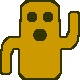
\includegraphics[width=100pt]{haniwa-d-u.jpg}
\end{figure}

\bibliographystyle{apalike} %参考文献出力スタイル
\bibliography{example_ref_JP.bib} %hoge.bibから拡張子を外した名前


\appendix

\section{付録セクション}

テスト．



\end{document}